\documentclass[12pt]{article}

\usepackage{amsmath}
\usepackage{amssymb}
\usepackage{bm}
\usepackage{enumerate}
\usepackage{fancyvrb}
\usepackage[top=1in, bottom=1in, left=1in, right=1in]{geometry}
\usepackage{hyperref}
\usepackage{placeins}
\usepackage{tikz}
\usepackage{tikzsymbols}
\usepackage{todonotes}
\usepackage{bbm}
\usepackage{color}
\newcommand{\rmn}[1]{{\textcolor{blue}{\bf [{\sc rmn:} #1]}}}
\DeclareMathOperator*{\argmax}{arg\,max}

\usetikzlibrary{positioning,calc}
%%%%%%%%%
\usepackage[most]{tcolorbox}
\newtcolorbox[]{solution}[1][]{%
    breakable,
    enhanced,
    colback=white,
    title=Solution,
    #1
}
%%%%%%%%%%
\title{10-703 Deep Reinforcement Learning and Control\\
  Assignment 2: Model-Free Learning\\
  Spring 2018\\
}

\date{Febuary 21, 2018\\
  \hspace{1cm}\\
Due March 7, 2018}

\begin{document}

\maketitle

\section*{Instructions}

You have around 15 days from the release of the assignment until it is due. Refer to Grade-scope for the exact time due.  You may work in teams of \textbf{2} on this assignment. Only one person should submit the writeup and code on Gradescope. Additionally you should upload your code to Autolab, please make sure the same person who submitted the writeup and code to Gradescope is the one who submits it to Autolab.  Make sure you mark your partner as a collaborator on Gradescope (You do not need to do this in Autolab) and that both names are listed in the writeup.  Writeups should be typeset in Latex and submitted as PDF. All code, including auxiliary scripts used for testing should be
submitted with a README.

\section*{Introduction}

% what is the goal of this section.
In Homework 1, you learned about and implemented various model-based techniques to solve MDPs. These ``planning'' techniques work well when we have access to a model of the environment; however getting access to such a model is often unfeasible. In this Homework, you will explore an alternative to the model-based regime, i.e. model-free learning. 
In particular, you will learn about Temporal Difference learning and its variants, and implement a version of TD learning called Q-learning. We will look at implementing Q learning with both tabular methods and deep function approximators. 

You will work with the OpenAI Gym environments, and learn how to train a Q-network from state inputs on a gym environment. The goal is to understand and implement some of the techniques that were found to be important in practice to stabilize training and achieve better performance. We also expect you to get comfortable using Tensorflow or Keras to experiment with different architectures, and understand how to analyze your network's final performance and learning behavior. 

Please write your code in the file \texttt{DQN\_Implementation.py}, the template code provided inside is just there to give you an idea on how you can structure your code but is not mandatory to use.

\section*{Background in Q-learning and Variants}

Function approximators have proved to be very useful in the reinforcement learning setting. Typically, one represents Q-functions using a class of parametrized function approximators $\mathcal Q = \{ Q _w \mid w \in \mathbb R ^p \}$, where $p$ is the number of parameters. Remember that in the \emph{tabular setting}, given a $4$-tuple of sampled experience $(s, a, r, s')$, the vanilla Q-learning update is 
%% is for a pair (s, a, r, s')
\begin{align}
	Q(s, a) := Q(s, a) + 
		\alpha \left( 
			r + \gamma \max _{a' \in A} Q(s', a') 
				- Q(s, a) 
		\right)   ,
	\label{eq:tab_qlearn}
\end{align}
where $\alpha \in \mathbb R$ is the learning rate. In the \emph{function approximation setting}, the update is similar: 
\begin{align}
	w := w + 
		\alpha \left( 
			r + \gamma \max _{a' \in A} Q _w(s', a') 
				- Q _w(s, a) 
		\right) \nabla _w 
			Q _w (s, a) .
	\label{eq:fapp_qlearn}
\end{align}
% this part is kind of unnecessary.
Q-learning can be seem as a 
pseudo stochastic gradient descent step on 
\begin{align*}
	\ell (w) = \mathbb E _{s, a, r, s'} 
		\left( 
			r + \gamma \max _{a' \in A} Q _w(s', a')
				- Q _w(s, a) 
		\right) ^2 ,
\end{align*}
where the dependency of $\max _{a' \in A} Q _w(s', a')$ on $w$ is ignored, i.e., it is treated as a fixed target. Many of the methods that you will implement in this homework are variants of update \eqref{eq:fapp_qlearn}. We recommend reading through the \emph{deep Q-learning implementation} described in~\cite{mnih2013playing, mnih2015human}. 

% BEGIN comment out Double DQN
\iffalse 
% namely in the way the targets are constructed and maintained.
maintains two Q-networks: the online network, which plays the same role of the $Q _w$ terms  $Q _w(s, a)$ and $\nabla _w Q _w (s, a)$ in update~\eqref{eq:fapp_qlearn}, and the target network, which is used in the target in update~\eqref{eq:fapp_qlearn}. The update in this case is 
\begin{align}
	w := w + 
		\alpha \left( 
			r + \gamma \max _{a' \in A} Q _{w ^-} (s', a') 
				- Q _w(s, a) 
		\right) \nabla _w 
			Q _w (s, a) .
\end{align}
The target Q-network is assigned every so often to be equal to the online Q-network, and is kept frozen until the next assignment. This helps the stability of the learning procedure, as with deep learning function approximators, updating the target Q-network with every update to the online Q-network proves too unstable. 

\emph{Double Q-learning}~\cite{van2016deep} also maintains two Q-networks, but they do not play a fixed role as online and target networks as in~\cite{mnih2013playing, mnih2015human}. Let us call the networks $Q _{w _1}$ and $Q _{w _2}$; at each update step, we flip a fair coin and either do 
\begin{align}
	{w _1} := {w _1} + 
		\alpha \left( 
			r + \gamma Q _{w _2}
				(
					s', \argmax _{a' \in A} Q _{w _1} (s', a')
				) 
				- Q _{w _1}(s, a) 
		\right) \nabla _{w _1} 
			Q _{w _1} (s, a) 
\end{align}
or 
\begin{align*}
	{w _2} := {w _2} + 
		\alpha \left( 
			r + \gamma Q _{w _1}
				(
					s', \argmax _{a' \in A} Q _{w _2} (s', a')
				) 
				- Q _{w _2}(s, a) 
		\right) \nabla _{w _2} 
			Q _{w _2} (s, a) .	
\end{align*}
As at each update the role of $Q _{w _1}$ and $Q _{w _2}$ is determined stochastically with probability $0.5$, these networks play a symmetric role. This helps with the over-optimism of the targets in update~\eqref{eq:fapp_qlearn}.
\fi
% END of comment out Double DQN

In this homework, we will also ask you to implement the \emph{dueling deep Q-network} described in~\cite{wang2015dueling}. This amounts to a slightly different Q-network architecture from the 
one in~\cite{mnih2013playing, mnih2015human}. Most models will be trained using \emph{experience replay}~\cite{mnih2013playing, mnih2015human}, meaning that the $4$-tuples $(s, a, r, s')$ will be sampled from the replay buffer rather than coming directly from the online experience of the agent.

\section{Theory Questions}
\subsection*{Question 1.a \textbf{[5pts]}}

Consider a sequence of streaming data points $\mathbf{X}: \{ x_1, x_2, x_3, ... x_N\}$. At any given time instant $k$, one has access to data points $\{ x_1, x_2, ... x_k\}$; but not $\{ x_{k+1}, ... x_N\}$. 
Prove that the mean $\mu_k$ of the available data may be computed incrementally (online) at every time step $k$, in the form: $\mu_k =\mu_{k-1} + f(\mu_{k-1}, x_k)$.\\

\noindent
\begin{solution}
\end{solution}

\subsection*{Question 1.b \textbf{[5pts]}}
The function $f(x_k, \mu_{k-1})$ represents the error between the current estimate of the mean, $\mu_{k-1}$, and the true mean at time $k$, $\mu_k$. Consider the following scenario - an agent follows some policy in its environment, and receives a return $G_t$ from an episode starting at state $s_t$. We would like to update the value of state $s_t$, $V(s_t)$, using the newly obtained $G_t$. 

\begin{itemize}
    \item Treating the update of $V(s_t)$ as an online learning problem, where $G_t$ is the newly received data point, show that the current estimate of the value of the state $V(s_t)$ can be updated in a form analogous to Question 1.a. You may assume that the state $s_t$ has been visited $N(s_t)$ number of times.
    
    \item What is the error function $f$? What does the update you derived resemble?  
\end{itemize}

\noindent
\begin{solution}
\end{solution}

\subsection*{Question 1.c \textbf{[5pts]}}
The update you derived in Question 1.b is based on the return from the entire episode, $G_t$. However, this method only learns from the end of the episode. Instead, it is possible to accelerate the learning process by bootstrapping. 

\begin{enumerate}
    \item Consider the agent is in state $s_t$, takes an action $a_t$, and transitions to state $s_{t+1}$, receiving reward $r$. Write out the estimate of the return of this episode based on this reward $r$ and the current estimate of the value function $V$. 
    \item In the update from Question 1.b, replace the return $G_t$ with the above estimate of return, and write out the new update for the value function $V(s_t)$. What does this update resemble?
\end{enumerate}

\noindent
\begin{solution}
\end{solution}


\subsection*{Question 2.a \textbf{[5pts]}}
Update~\ref{eq:tab_qlearn} defines the TD update when the representation of the states and actions are in tabular form. Show that for a certain construction of the feature function $\phi$, the tabular representation representation is a special case of the TD update~\ref{eq:fapp_qlearn} where the function in $\mathcal Q$ is of the form $Q _w(s, a) = w ^T \phi(s, a)$. Give detailed description about your feature function and your proof for equivalence to earn full credits. \\

\noindent
\begin{solution}
TD update 2 is:
\begin{align}
w := w + 
		\alpha \left( 
			r + \gamma \max _{a' \in A} Q _w(s', a') 
				- Q _w(s, a) 
		\right) \nabla _w 
			Q _w (s, a) \\
\end{align}
Taking transpose on both sides:
\begin{align}
w^T = w^T + 
		\alpha \left( 
			r + \gamma \max _{a' \in A} Q _w(s', a') 
				- Q _w(s, a) 
		\right) \nabla _w 
			Q_w^T (s, a) \\
\end{align}
Now,
\begin{align}
Q_w(s, a) = w ^T \phi(s, a) \implies \nabla _w Q_w^T (s, a) = \phi^T(s,a) \\
w^T = w^T + 
		\alpha \left( 
			r + \gamma \max _{a' \in A} Q _w(s', a') 
				- Q _w(s, a) 
		\right) \phi^T(s,a) \\
\end{align}
Post-multiplying both sides by $\phi(s,a)$
\begin{align}
w^T\phi(s,a) = w^T\phi(s,a) + 
		\alpha \left(r + \gamma \max _{a' \in A} Q _w(s', a') - Q_w(s, a) \right) \phi^T(s,a)\times \phi(s,a) \\
\implies Q_w(s, a) = Q_w(s, a) + 
		\alpha \left(r + \gamma \max _{a' \in A} Q _w(s', a') - Q_w(s, a) \right) \phi^T(s,a)\times \phi(s,a)
\end{align}
Comparing equation 11 with the TD update 1, both equations are equal when $ \phi^T(s,a)\times \phi(s,a) = 1$. Hence, for all construction of feature function $\phi$ such that $\phi^T \phi =1$, the tabular representation is same as TD update 2.
\end{solution}

\subsection*{Question 2.b \textbf{[5pts]}}
State aggregation improves generalization by grouping states together, with one table entry used for each group. Let $\mathcal{X}: s \to x$ be the grouping function that maps a input state $s$ to its group $x$ and usually, the number of groups $|X| \ll |S|$. During training, whenever a state in a group is encountered, the groups' entry and the action $a$ is used to determine the state's value, and when the state is updated, the group's entry is updated. Assume $\mathcal Q$ is still in the the form $Q _w(s, a) = w ^T \phi(s, a)$. Show that a tabular representation with state aggregations is also a special case of TD update~\ref{eq:fapp_qlearn} under certain construction of feature function $\phi$. Give detailed description about your feature function and your proof for equivalence to earn full credits. 

\noindent

\begin{solution}
TD update 2 is:
\begin{align*}
w := w + 
		\alpha \left( 
			r + \gamma \max _{a' \in A} Q _w(s', a') 
				- Q _w(s, a) 
		\right) \nabla _w 
			Q _w (s, a) \\
\end{align*}
Taking transpose on both sides:
\begin{align*}
w^T = w^T + 
		\alpha \left( 
			r + \gamma \max _{a' \in A} Q _w(s', a') 
				- Q _w(s, a) 
		\right) \nabla _w 
			Q_w^T (s, a) \\
\end{align*}
Now, let the probability of aggregation is represented as $P(x|s)$ which is probability that state $s$ will will be grouped in group $x$
\begin{align*}
Q_w(s, a) = w ^T \phi(s, a) = \sum_x w ^T P(x|s) \phi(x)\\
\implies \nabla _w Q_w^T (s, a) = \sum_x P(x|s) \phi^T(s,a) \\
w^T = w^T + 
		\alpha \left( 
			r + \gamma \max _{a' \in A} Q _w(s', a') 
				- Q _w(s, a) 
		\right) (\sum_x P(x|s) \phi^T(s,a)) \\
\end{align*}
Post-multiplying both sides by $\sum_x\phi(x) P(x|s)$
\begin{align}
w^T \sum_x P(x|s) \phi(s,a) = w^T \sum_x P(x|s) \phi(s,a) + \nonumber \\ \nonumber
		\alpha \left(r + \gamma \max _{a' \in A} Q _w(s', a') - Q_w(s, a) \right) \sum_x P(x|s) \phi^T(s,a)\times \sum_x P(x|s) \phi(s,a) \\
\end{align}
Comparing equation 12 with the TD update 1, both equations are equal when $ \sum_x P(x|s) \phi^T(s,a)\times \sum_x P(x|s) \phi(s,a) = 1$.  
\end{solution}


\section{Programming Questions}
Before starting your implementation, make sure you have the environments correctly installed.
For this assignment you will solve Cartpole (\texttt{Cartpole-v0}) and Mountain Car-v0 (\texttt{MountainCar-v0}). For extra-credit \textbf{[+10pts]}, you will need to additionally solve the more challenging Space Invaders (\texttt{SpaceInvaders-v0}) environment. For all of the following implementations we would like you to document your findings in the writeup as described after the questions.

Try to keep your implementation modular. Once you have the basic DQN working it will only be a little bit of work to get DQN and dueling networks working. Please write your code in the file \texttt{DQN\_implementation.py}, the template code provided inside is just there to give you an idea on how you can structure your code but is not mandatory to use.

\begin{enumerate}

    \item\textbf{[20pts]} Implement a linear Q-network (no experience replay, i.e. experience is sampled directly from the environment online). Train your network (separately) on both the \texttt{CartPole-v0} environment and the \texttt{MountainCar-v0} environment. Use the full state of each environment (such as angular displacement and velocity in the case of Cartpole) as inputs.
              
    In case of the simple environments, you may observe good performance even with a linear Q-network. If you can get this running you will have understood the basics of the assignment. 
    
    For this question, look at the \texttt{QNetwork} and \texttt{DQN\_Agent} classes in the code. You will have to implement the following: 
    \begin{itemize}
        \item Create an instance of the Q Network class.
        \item Create a function that constructs a policy from the Q values predicted by the Q Network - both epsilon greedy and greedy policies.
        \item Create a function to train the Q Network, by interacting with the environment.
        \item  Create a function to test the Q Network's performance on the environment.
    \end{itemize}
    
    Are you able to solve both environments with a linear network? Why or why not? 

    \item \textbf{[15pts]} Implement a linear Q-network with experience replay. Use the experimental setup of~\cite{mnih2013playing, mnih2015human} to the extent possible. Use this as an opportunity to work out any bugs with your replay memory.
    
    You can refer to the \texttt{Replay\_Memory} class in the code. You may need the following functions: 
    \begin{itemize}
        \item Appending a new transition from the memory. 
        \item Sampling a batch of transitions from the memory to train your network. 
        \item Initially burn in a number of transitions into the memory. 
        \item You will also need to modify your training function of your network to learn from experience sampled \textit{from the memory}, rather than learning online from the agent. 
    \end{itemize}
              
    As above, train your network (separately) on both the \texttt{CartPole-v0} environment and the \texttt{MountainCar-v0} environment. Does adding experience replay improve learning? 
             
	\item \textbf{[20pts]} Implement a deep Q-network, similar to that described in~\cite{mnih2013playing, mnih2015human}. While these papers use a convolutional architecture to address the image based state representation of Atari environments, a multi-layer Perceptron with $3$ hidden units should suffice for the environments. 
	
	Document any changes to your training procedure, optimization, etc. that you make to train your deep Q-network, as compared to the linear case. How does using this deep Q-network affect performance, convergence rate, and stability of training on both \texttt{Cartpole-v0} and \texttt{MountainCar-v0}?
	
	You may use the cluster to train this agent \textit{once you have worked out the bugs}, although these environments are simple enough that you may solve them on your own laptop in a few hours. 
	
    \item \textbf{[15pts]} Implement the dueling deep Q-network as described in~\cite{wang2015dueling}.
    Train your network (separately) on both the \texttt{CartPole-v0} environment and the \texttt{MountainCar-v0} environment. How does adding the two stream architecture affect performance? 
    
    \item \textbf{Extra Credit: [+10 pts]}  Implement a deep Q-network (dueling deep Q-network not required) using a convolutional architecture to solve the \texttt{SpaceInvaders-v0} environment. Train your network by passing in $4$ consecutive frames from the environment, as described in \cite{mnih2015human, mnih2013playing}. 
    
    Modify your replay memory to store images, preprocess them as necessary (resizing / normalization, etc.), and sample frames to provide to the network for training. You may find it necessary to implement a Target Q Network (as in the double Q learning paper \cite{van2016deep}) to stabilize training of the networks. Document these changes in your report.
    
    
\end{enumerate}

\noindent
\textbf{5pts} out of the total of \textbf{100pts} are reserved for overall report quality.

\textbf{For each of the above questions}, we want you to generate a \emph{performance plot across time}.  To do this, you should periodically run (e.g., every $10000$ or $100000$ updates to the Q-network) the policy induced by the current Q-network for $20$ episodes and average the total reward achieved. Note that in this case we are interested in total reward without discounting or truncation. During evaluation, you should use a tinier $\epsilon$ value in your $\epsilon$-greedy policy. We recommend $0.05$. The small amount of randomness is to prevent the agent from getting stuck.  Also briefly comment on the training behavior and whether you find something unexpected in the results obtained.

Additionally, for each of the models, we want you to generate a \emph{video capture} of an episode played by your trained Q-network at different points of the training process ($0/3$, $1/3$, $2/3$, and $3/3$ through the training process) of both environments, i.e. \texttt{Cartpole-v0} and \texttt{MountainCar-v0}. 

An episode is defined as $200$ successful time steps in Cartpole, and reaching the top of the mountain in Mountain Car. You can use the \texttt{Monitor} wrapper to generate both the performance curves (although only for $\epsilon$-greedy in this case) and the video captures. Look at the OpenAI Gym tutorial for more details on how to use it. We recommend that you periodically checkpoint your network files and then reload them after training to generate the evaluation curves. It is recommended you do regular checkpointing anyways in order to ensure no work is lost if your program crashes.

Finally, construct a \emph{table} with the average total reward per episode in $100$ episodes
achieved by your fully trained model. Also show the information about the standard deviation, i.e., 
each entry should have the format $\text{mean} \pm \text{std}$.
There should be an entry per model. Briefly comment on the results of this table.

We recommend you to follow closely the hyperparameter setup described below, or as in the references for training on the image based environment. Even if you fully replicate the experimental from the paper, we expect you to summarize it briefly in the report once. After that you can simply describe differences from it and mention that you used the same experimental setup otherwise if that was the case.

You should submit  your report, video captures, and code through Gradescope. Your code should be 
reasonably well-commented in key places of your implementation. Make sure your code also has a README file.

\section*{Guidelines on references}
We recommend you to read all the papers mentioned in the references. There is a significant overlap between different papers, so in reality you should only need certain sections to implement 
what we ask of you. We provide pointers for relevant sections for this assignment for your convenience

The work in~\cite{mnih2013playing} contains the description of the experimental setup. Read paragraph~3 of section~4 for a description of the replay memory; read Algorithm~1; read  paragraphs~1 and~3 of section~4.1 for preprocessing and model architecture respectively; read section~5 for the rest of the experimental setup (e.g., reward truncation, optimization algorithm, exploration schedule,
and other hyperparameters). The methods section in~\cite{mnih2015human}, may clarify a few details
so it may be worth to read selectively if questions remain after reading~\cite{mnih2013playing}.

In~\cite{wang2015dueling}, look at equation~11 and read around three paragraphs up and down for how to set up the dueling architecture; read paragraph~2 of section~4.2 for comments on the experimental setup 
and model architecture. It may be worth to skim additional sections of all these papers. 

\section*{Guidelines on hyperparameters}

In this assignment you will implement improvements to the simple update Q-learning formula that make learning more stable and the trained model more performant. We briefly comment on the meaning of each hyperparameter and some reasonable values for them.
\begin{itemize}
	\item Discount factor $\gamma$: $1.$ for MountainCar, and $0.99$ for CartPole and Space Invaders. 
	\item Learning rate $\alpha$: $0.0001$; typically a schedule is used where learning rates get increasingly smaller. 
    \item Exploration probability $\epsilon$ in $\epsilon$-greedy: 
    While training, we suggest you start from a high epsilon value, and anneal this epsilon to a small value ($0.05$ or $0.1$) during training. 
    We have found decaying epsilon linearly from $0.5$ to $0.05$ over $100000$  iterations works well. 
    During test time, you may use a greedy policy, or an epsilon greedy policy with small epsilon ($0.05$).
    
	\item Number of training sampled interactions with the environment: 
	For MountainCar-v0, we recommend training for $3000$ to $5000$ episodes, though you should see improvements much before this. For CartPole-v0
	, train for $1000000$ iterations. 
	
	Look at the average reward achieved in the last few episodes  to test if performance has plateaued; it is usually a 
    good idea to consider reducing the learning rate or the exploration 
	probability if performance plateaus.
 	
 	\item Replay buffer size: $50000$; 
	this hyperparameter is used only for experience replay. It determines how many of the last transitions experienced you will keep in the replay buffer before you start rewriting this experience with more recent transitions. \textbf{(For Extra Credit:) } Use a replay buffer size of $1000000$.
	
	\item Batch size:  32;  typically, rather doing the update as in (2), we use a small batch ofsampled experiences from the replay buffer; this provides better hardware utilization.
	
 	\item \textbf{(For Extra Credit:) }Number of frames to feed to the Q-network: $4$; as a single frame may not be a good representation of the current state. 
% 		cannot tell if the spaceships are moving left or right), 
    Multiple frames are fed to the Q-network to compute the Q-values; note that in this case, the state effectively is a list of last few frames.
    
    \item \textbf{(For Extra Credit:) } Input  image  resizing:  Using the original input size of 210x160x3 is computationally expensive. Instead, you may resize the image input to 84x84x3 to make it more manageable. Further, you may convert the RGB image to a Grayscale image.
    

\end{itemize}

In addition to the hyperparameters you also have the choice of which
optimizer and which loss function to use. We recommend you use Adam as
the optimizer. It will automatically adjust the learning rate based on
the statistics of the gradients its observing. Think of it like a
fancier SGD with momentum. Both Tensorflow and Keras provide versions
of Adam.

For the loss function, you can use Mean Squared Error - if you are doing so, \textbf{please demonstrate} how the vanilla Q-learning update is equivalent to minimizing a quadratic loss function. 

The implementations of the methods in this homework have multiple
hyperparameters.  These hyperparameters (and others) are part of the
experimental setup described in~\cite{mnih2013playing, mnih2015human}.
For the most part, we strongly suggest you to follow the experimental
setup described in each of the papers.  \cite{mnih2013playing,
  mnih2015human} was published first; your choice of hyperparameters
and the experimental setup should follow closely their setup.
\cite{van2016deep, wang2015dueling} follow for the most part the setup
of \cite{mnih2013playing, mnih2015human}.  We recommend you to read
all these papers.  We give pointers for the most relevant portions for
you to read in a future section.

\section*{Guidelines on implementation}

This homework requires a significant implementation effort. It is hard to read through the papers once and know immediately what you will need to be implement. We suggest you to think about the different components (e.g., replay buffer, Tensorflow or Keras model definition, model updater, model runner,
exploration schedule, learning rate schedule, ...) that you will need to implement for each of the different methods that we ask you about, and then read through the papers having these components in mind. By this we mean that you should try to divide and implement small components with well-defined functionalities rather than try to implement everything at once. Much of the code and experimental setup is shared between the different methods so identifying well-defined reusable components will 
save you trouble. We provide some code templates that you can use if you wish. Contrary to the previous assignment, abiding to the function signatures defined in these templates is not mandatory you can write your code from scratch if you wish. 

Please note, that while this assignment has a lot of pieces to implement, most of the algorithms you will use in your project will be using the same pieces. Feel free to reuse any code you write for your
homeworks in your class projects.


This is a challenging assignment. 
\textbf{Please start early!}


\nocite{*}
\bibliographystyle{plain}
\bibliography{deeprlhw2}


\newpage
\textbf{Write-up for implementation section: }
\begin{enumerate}
\item Linear Q Network
\item Linear Q Network with replay: For Mountain Car,  Figure~\ref{fig:MountainCar_linear_replay_reward} shows that learning is unstable. But we can terminate the training when we start getting good results. Here we stop the training at 320,016 iteration which is the end of the training and is making the car reach the flag but we could have terminated the training anywhere else as well.

\begin{figure}[h]
  \centering
  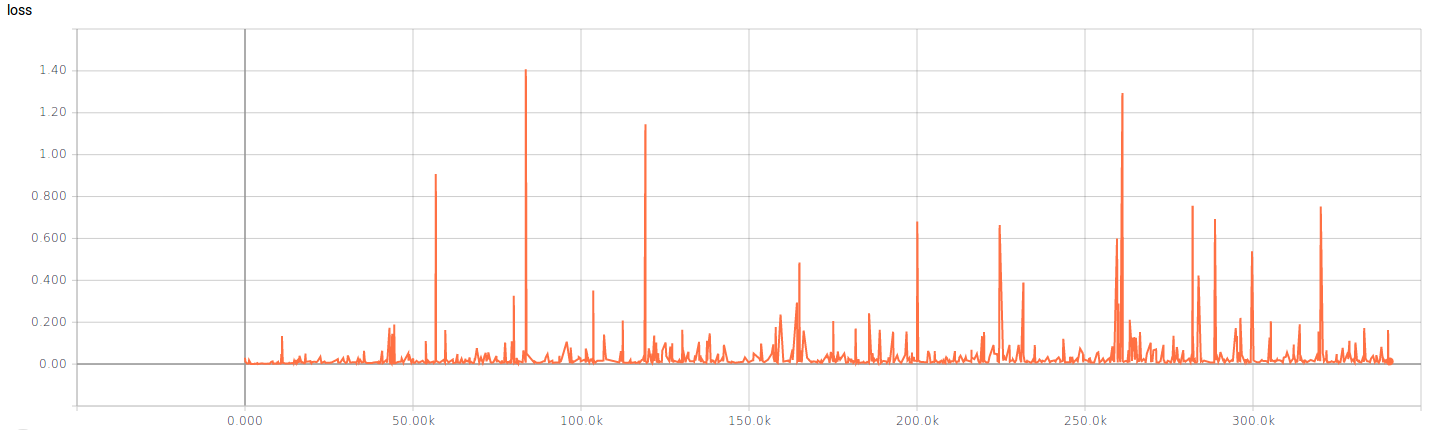
\includegraphics[width=1\textwidth]{figures/MountainCar_linear_replay_loss.png}
  \caption{\label{fig:MountainCar_linear_replay_loss} Loss tracking (every iteration) during training with Deep Q Network for \texttt{MountainCar-v0} environment.}
\end{figure}

\begin{figure}[h]
  \centering
  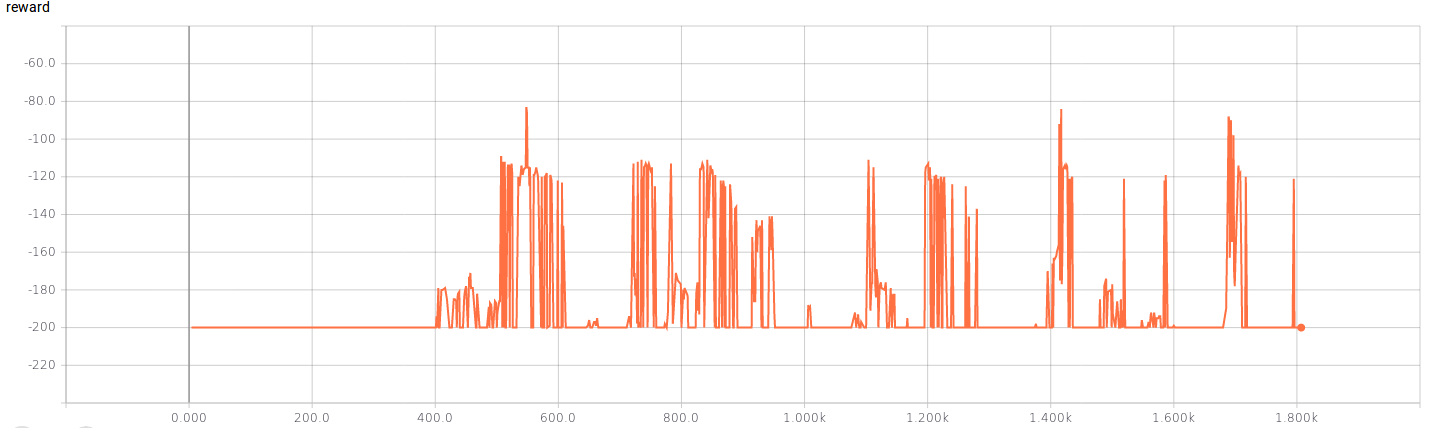
\includegraphics[width=1\textwidth]{figures/MountainCar_linear_replay_reward.png}
  \caption{\label{fig:MountainCar_linear_replay_reward} Reward tracking (every episode) during training with Deep Q Network for \texttt{MountainCar-v0} environment.}
\end{figure}CartPole

\item Deep Q Network: For both environment, DQN gave better rewards versus linear Q-Network for us. This makes sense as the model expected is non-linear and linear Q-Network can not learn the perfect policy. The final model used is the end of training which is 990,134 iteration for Mountain Car and 94490 iterations for Cart-Pole environment.
\begin{figure}[h]
  \centering
  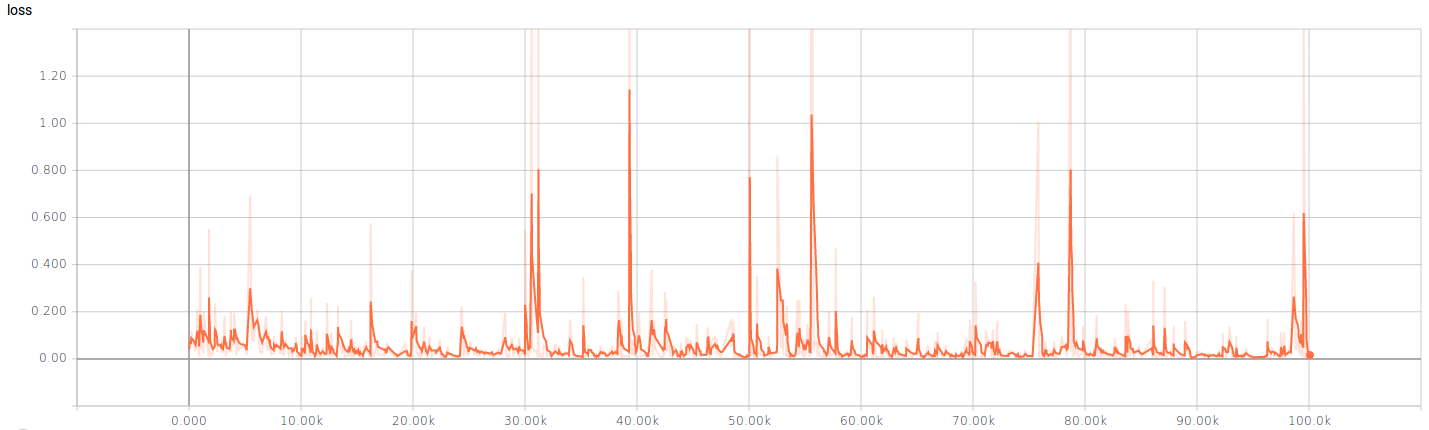
\includegraphics[width=1\textwidth]{figures/CartPole_DQN_replay_loss.png}
  \caption{\label{fig:CartPole_DQN_replay_loss} Loss tracking (every iteration) during training with Deep Q Network for \texttt{CartPole-v0} environment.}
\end{figure}

\begin{figure}[h]
  \centering
  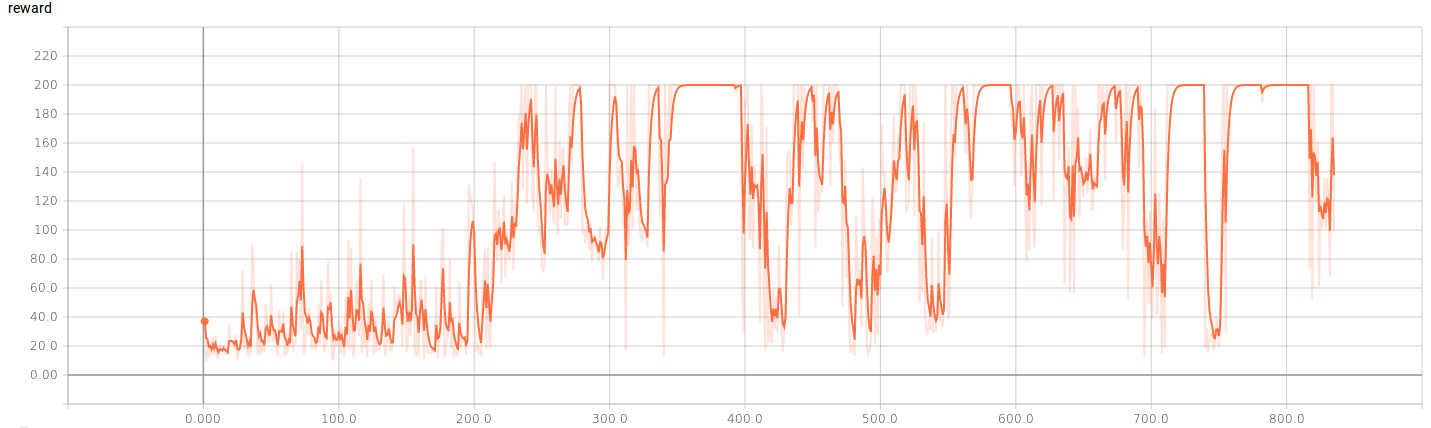
\includegraphics[width=1\textwidth]{figures/CartPole_DQN_replay_reward.png}
  \caption{\label{fig:CartPole_DQN_replay_reward} Reward tracking (every episode) during training with Deep Q Network for \texttt{CartPole-v0} environment.}
\end{figure}

\begin{figure}[h]
  \centering
  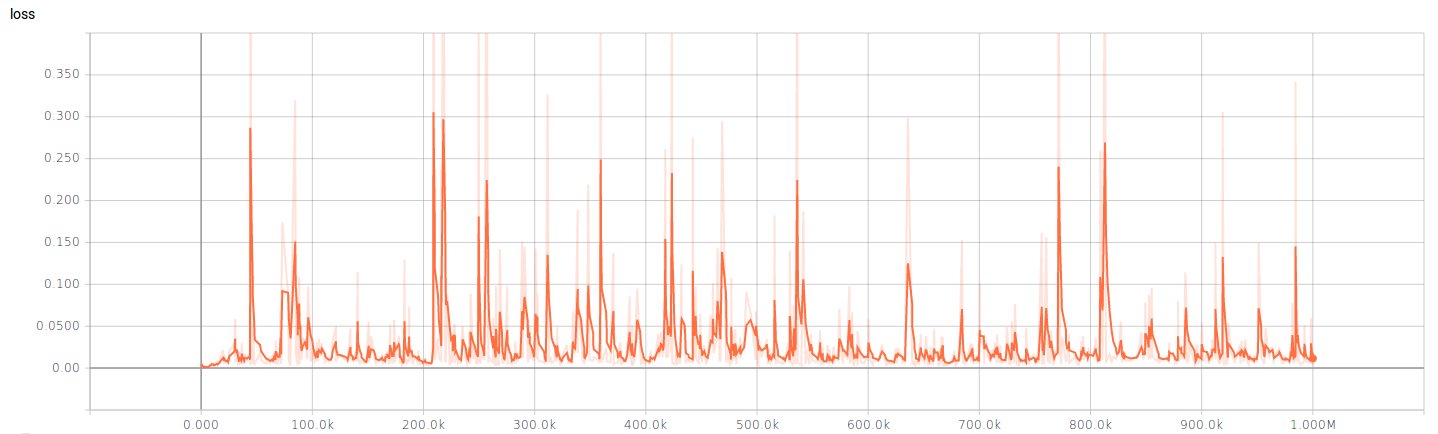
\includegraphics[width=1\textwidth]{figures/MountainCar_DQN_replay_loss.png}
  \caption{\label{fig:MountainCar_DQN_replay_loss} Loss tracking (every iteration) during training with Deep Q Network for \texttt{MountainCar-v0} environment.}
\end{figure}

\begin{figure}[h]
  \centering
  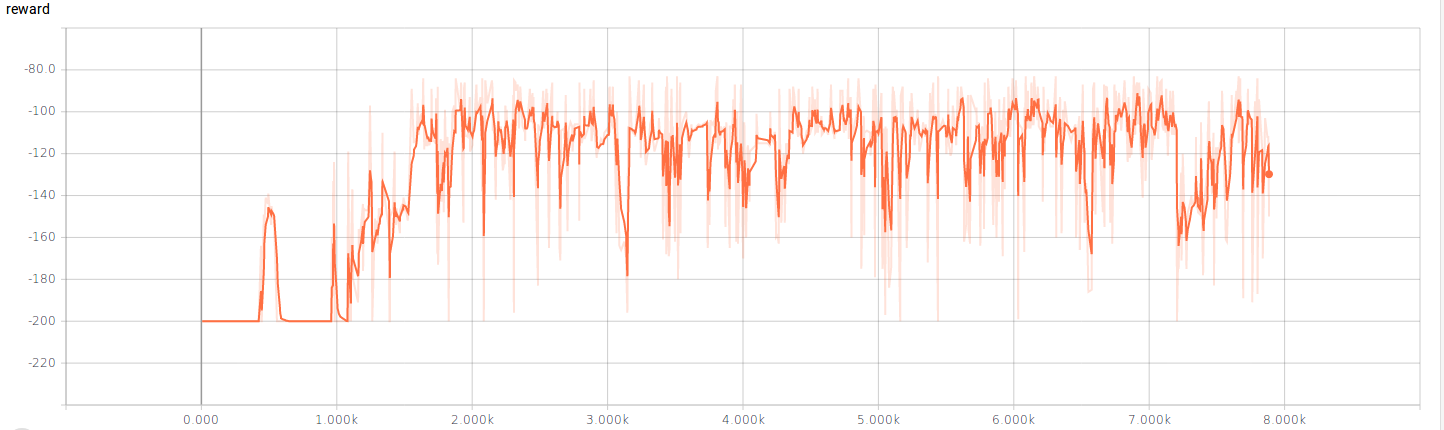
\includegraphics[width=1\textwidth]{figures/MountainCar_DQN_replay_reward.png}
  \caption{\label{fig:MountainCar_DQN_replay_reward} Reward tracking (every episode) during training with Deep Q Network for \texttt{MountainCar-v0} environment.}
\end{figure}
\FloatBarrier



\item Duelling Deep Q Network: \\ 
For Mountain Car, looking at  Figure~\ref{fig:MountainCar_DQN_duelling_replay_reward}, we again see unstable learning and this time decided to take the model saved during the training and not the end of training as shown in the Figure~\ref{fig:MountainCar_DQN_duelling_replay_reward}. We are taking the model after 134563 iteration giving us good reward of $-173$ which is worse that DQN results but this is mainly because we did not find the right combination of hyper parameters. We believe that Duelling DQN should give equivalent or even better results if compared with DQN.
\begin{figure}[h]
  \centering
  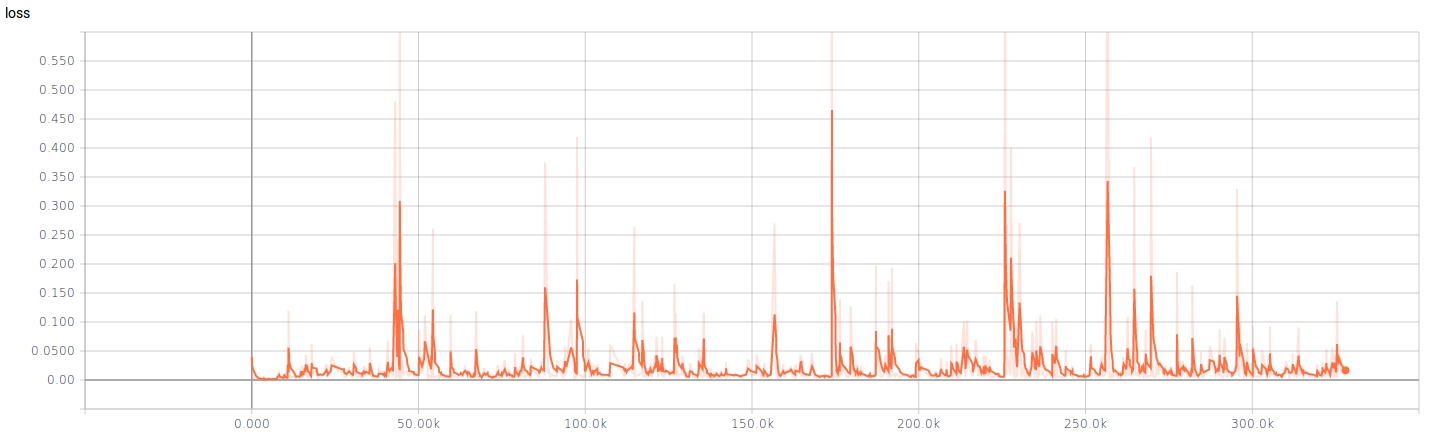
\includegraphics[width=1\textwidth]{figures/MountainCar_DQN_duelling_replay_loss.png}
  \caption{\label{fig:MountainCar_DQN_duelling_replay_loss} Loss tracking (every iteration) during training with Deep Q Network for \texttt{MountainCar-v0} environment.}
\end{figure}

\begin{figure}[h]
  \centering
  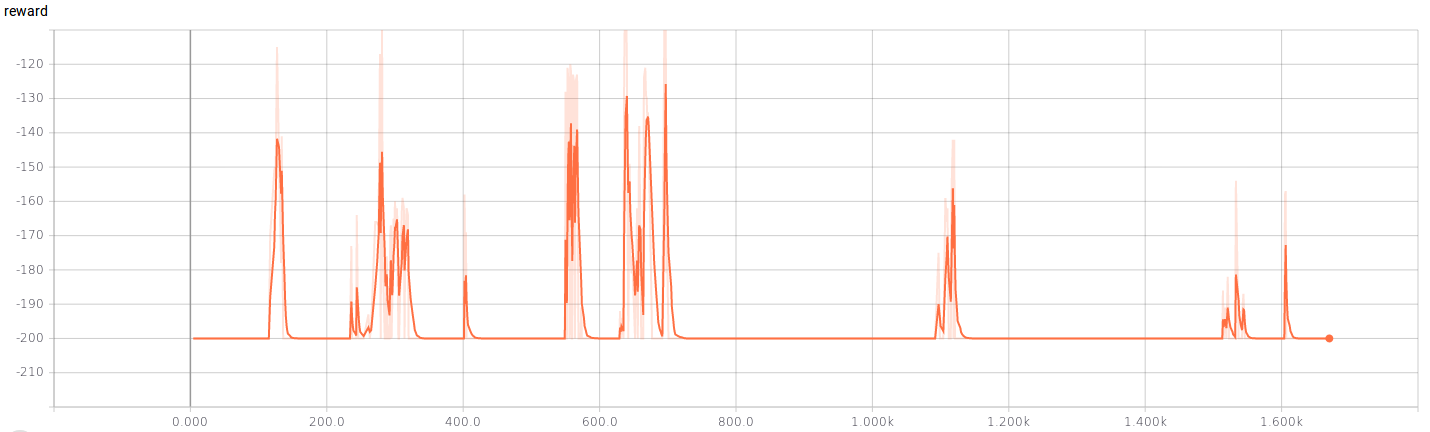
\includegraphics[width=1\textwidth]{figures/MountainCar_DQN_duelling_replay_reward.png}
  \caption{\label{fig:MountainCar_DQN_duelling_replay_reward} Reward tracking (every episode) during training with Deep Q Network for \texttt{MountainCar-v0} environment.}
\end{figure}
\FloatBarrier

For Cart-pole, looking at  Figure~\ref{fig:CartPole_DQN_duelling_replay_reward}, we do not see convergence. We are taking the model after 94142 iteration giving us good reward of only $9$ which is worse that DQN results but this is mainly because we did not find the right combination of hyper parameters.
\begin{figure}[h]
  \centering
  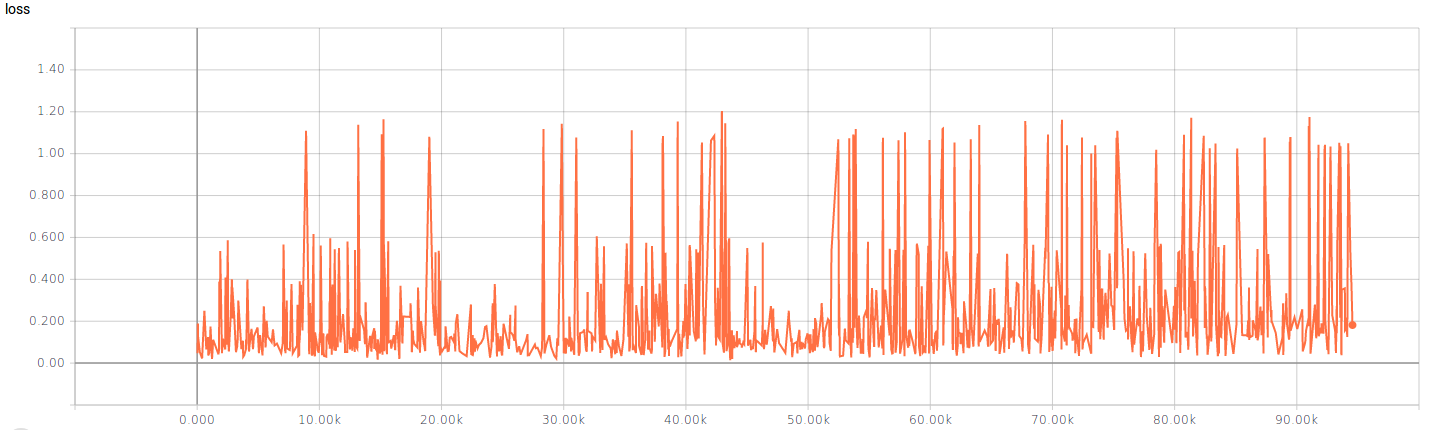
\includegraphics[width=1\textwidth]{figures/CartPole_DQN_duelling_replay_loss.png}
  \caption{\label{fig:CartPole_DQN_duelling_replay_loss} Loss tracking (every iteration) during training with Deep Q Network for \texttt{CartPole-v0} environment.}
\end{figure}

\begin{figure}[h]
  \centering
  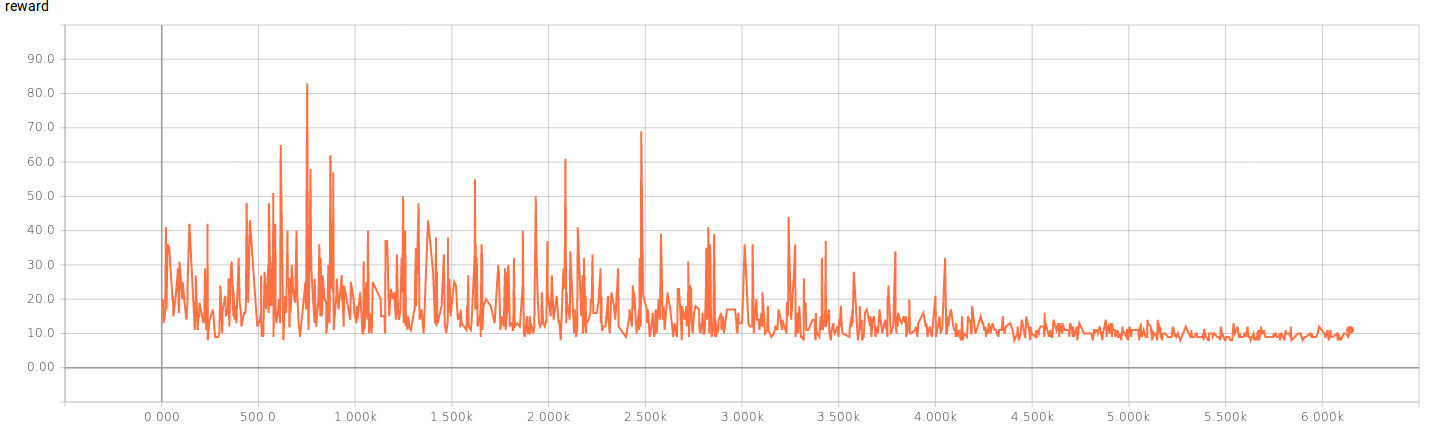
\includegraphics[width=1\textwidth]{figures/CartPole_DQN_duelling_replay_reward.png}
  \caption{\label{fig:CartPole_DQN_duelling_replay_reward} Reward tracking (every episode) during training with Deep Q Network for \texttt{CartPole-v0} environment.}
\end{figure}
\FloatBarrier

\end{enumerate}
\emph{table} with the average total reward per episode in $100$ episodes is attached below:
achieved by your fully trained model
\begin{center}
\begin{tabular}{|l||c|c|c|}\hline
	System & Description &Average reward & std. dev\\\hline
	Mountain Car & Epsilon greedy using linear Q-network and no replay & &\\ \hline
	Mountain Car & Epsilon greedy using linear Q-network with replay & -144.1 & 24.18 \\ \hline
	Mountain Car & Epsilon greedy using DQN with replay & -132.12 & 29.4\\ \hline
	Mountain Car & Epsilon greedy using duelling DQN with replay & -173 & 37.2\\ \hline
	
	Cart-pole & Epsilon greedy using linear Q-network and no replay & &\\ \hline
	Cart-pole & Epsilon greedy using linear Q-network with replay & &  \\ \hline
	Cart-pole & Epsilon greedy using DQN with replay & 192.57 & 36.58\\ \hline
	Cart-pole & Epsilon greedy using duelling DQN with replay & 9.32 & .82\\ \hline
\end{tabular}
\end{center}

\end{document}

